\chapter{Introduction and Theory Overview} \label{chap:1}

\section{Introduction}
The analysis aims at searching for heavy resonances decaying to a pair of Higgs
bosons in the four b quark final state using 35.9$fb^{-1}$ proton-proton collision data at center-of-mass energy 13 TeV collected with the CMS detector at the LHC. Figure~\ref{fig:test} shows the Feynman diagram of the channel. 

The Higgs tagging process uses the b-tagging algorithm, N-subjettiness variable, and the mass of the jets. The analysis is searching for a bump in the dominant background of multi-jet events.


\begin{figure}[t]
  \begin{center}

    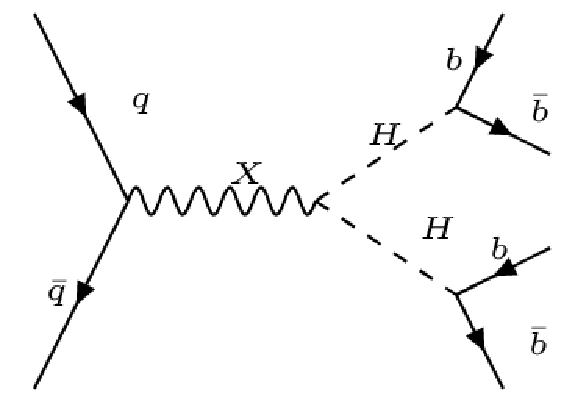
\includegraphics[width=0.5\textwidth]{Figures/Screenshot_20170601_160641.pdf} 
    \end{center}
  \caption{The Feynman diagram of q$\bar{q}$ $\rightarrow$ X $\rightarrow$ HH $\rightarrow$ $b\bar{b}b\bar{b}$.}
  	
\end{figure}
\label{fig:test}

In Chapter \ref{chap:1}, an overview of Warped Extra Dimension theory, predicted particles, and motivation is presented. In Chapter \ref{chap:2}, the LHC and the CMS detector are introduced. In Chapter \ref{chap:3}, the information of the data and the Monte Carlo simulation is shown along with the comparison of shape of each discriminant variable. The reconstruction and event selection are also fully detailed. In Chapter \ref{chap:4}, the background estimation method based on data driven is presented. All systematic uncertainties considered are documented in Chapter \ref{chap:5}. Finally, the result of 95$\% $ CL$_{s}$ upper limit of cross section $\times$ branch ratio is shown in Chapter \ref{chap:6}. 

\section{Theory}
%http://dx.doi.org/10.1016/j.physletb.2012.08.021
%http://www.sciencedirect.com/science/article/pii/S037026931200857X

The discovery of the boson whose mass around 125 GeV and with properties close to Higgs mechanism in the standard model (SM) has incited the search under Higgs potential including Higgs self-coupling~\citep{jetarea_fastjet_pu,HiggsdiscoveryAtlas}. Especially, it is a channel worth exploring and finding new physic beyond the SM. 
Targeting heavy resonance, the model Warped Extra Dimension is considered. 

\subsection{Warped Extra Dimension} 

%https://journals.aps.org/prl/pdf/10.1103/PhysRevLett.83.3370
To solve the hierarchy problem, Warped Extra dimension proposed by Randall and Sundrum postulates a scenario that the SM particles and forces with the exception of gravity are confined to a four-dimensional subspace within (4+n)-dimensional space-time, referred to as "3-brane", 
to explain the fact that we do not see experimental signs of the extra dimensions~\citep{Randall:1999ee}.  The space-time matrix takes the form~\citep{Oliveira:2014kla}:

\begin{equation} 
\begin{split}
ds^2 = e^{-2\sigma(\phi)}\eta_{\mu\nu}dx^{\mu}dx^{\nu} + r^2_{c}d\phi^2, 
\end{split}
\end{equation}
where $\mu$ and $\nu$ run over 1, 2, 3, and 4, $\eta_{\mu\nu}$ is the standard basis for orthogonal vectors in Minkowski space, $\sigma$ is the "warp" factor, $r_{c}$ is the scale of the fifth dimension, and $\phi$ is the fifth dimension. Its classical action is 

\begin{equation}
\begin{split}
S = S_{Gravity}+S_{TeV}+S_{Planck}+S_{Matter},
\end{split}
\end{equation},
where $S_{Gravity}$ is the action of bulk gravity, $S_{TeV}$ is the action of visible sector field, $S_{Planck}$ represents hidden sector field, and $S_{Matter}$ is the action of matter field. The actions can be written as:

\begin{equation} 
\begin{split}
S_{TeV}=-\int d^4x \sqrt{g(\phi =0,\pi)}\Lambda_{TeV}\\
S_{Planck}=-\int d^4x \sqrt{g(\phi =0,\pi)}\Lambda_{Planck}\\
S_{Gravity}=\int d^4 \int ^{\pi}_{-\pi} d\phi \sqrt{g}(-\Lambda_{bulk}+2M^3_{5}R),
\end{split}
\end{equation}
where $\Lambda$ is the vacuum energy density, R is Ricci metrix, g is five-dimensional orthogonal matrix, and $M_5$ is five-dimensional Planck mass. We arrive at:

\begin{equation} 
\begin{split}
\sigma(\phi)=r_{c}|\phi | \sqrt{\frac{-\Lambda}{24M^2_5}}\equiv r_c|\phi |k \\
k\equiv  \sqrt{\frac{-\Lambda}{24M^2_5}}, \\
\end{split}
\end{equation}
where k is referred as curvature factor, and $\Lambda$ is the vacuum energy density, which should be negative from the negative term of potential energy. We can integrate the fifth dimension and get four-dimension Planck mass: 
\begin{equation} 
\begin{split}
\bar{M}^2_{Pl}=\frac{M^3_5}{k}(1=e^{-2\pi kr_c}).
\end{split}
\end{equation}

Finally, we get the space-time matrix:  
\begin{equation} 
\begin{split}
ds^2 = e^{-2kr_c\phi}\eta_{\mu\nu}dx^{\mu}dx^{\nu} + r^2_{c}d\phi^2, 
\end{split}
\end{equation}


where k is a scale of the order of the Planck scale, $x^{\mu}$ are
coordinates for the familiar four dimensions, while 0 $\leq$ $\phi$ $\leq$ $\pi$ is the coordinate for an extra dimension, which is
a finite interval whose size is set by $r_c$. The exponential is the source of large hierarchy between the weak scale and the observed Planck scale.  


%https://journals.aps.org/prl/pdf/10.1103/PhysRevLett.83.4922
%https://arxiv.org/pdf/hep-ph/9911406.pdf

%https://arxiv.org/pdf/hep-ph/9909255.pdf
%https://arxiv.org/pdf/hep-ph/0701186.pdf
%https://arxiv.org/pdf/hep-ph/0701150.pdf
There are models predicting the existence of new particles, such as spin-0 radion and spin-2 graviton~\citep{Davoudiasl:1999jd,Agashe:2007zd,Fitzpatrick:2007qr}. For example, a radion scalar is added to stabilize the $r_c$ in RS theory without a fine-tuning of parameters~\citep{Goldberger:1999uk}. One model proves that
a radion field can remove the constraints between two branes without a stabilized radius~\citep{Csaki:1999mp}, while another model holds that 
%https://arxiv.org/pdf/hep-th/0008151.pdf
a radion scalar can exist with radius stabilization in bulk scalar field while assuming stabilization exists~\citep{Csaki:2000zn}.
A possible mixing of the radion which is the only graviscalar in RS model and the Higgs boson is proposed~\citep{Giudice:2000av}.
%https://arxiv.org/pdf/hep-ph/0002178.pdf
However, according to the latest experimental data, the mixing is expected to be small. Therefore, the contribution of the mixing is not considered in this analysis~\citep{Desai:2013pga}.
%https://arxiv.org/pdf/1307.3765.pdf

We follow Ref.~\citep{Agashe:2013kyb} to calculate the cross section of bulk graviton, which inputs the coupling constant from the theory: 
\begin{equation} 
\begin{split}
gg \rightarrow KK graviton \rightarrow ZZ, WW, hh (and t\bar{t}, b\bar{b}) \\
\textit{L}_{prod.} = 0.053 (\frac{k}{M_{Pl}M_{G}})\eta^{\mu\alpha}\eta^{\nu\beta}h^{(1)}_{\alpha\beta}T^{gluon}_{\mu \nu}(x), 
\end{split}
\end{equation}
where the $M_G$ is the mass of KK graviton, and $T^{gluon}_{\mu \nu}$ is four-dimension four-momentum of SM gluon. The implementation of the calculation is described in Ref.~\citep{Oliveira:2014kla}. The model which is capable of calculating QCD induced spin-2 particle with the correction to next-to-leading-order is used. The cross section is calculated by \textsf{MG5\_aMC@NLO}.

Because of the Higgs-like property of radion, the cross section of radion is calculated by rescaling the cross section of the 125-GeV Higgs boson~\citep{Agashe:2013kyb,AN-16-300}. The production of Higgs-like particle by gluon-gluon fusion is followed by Ref.~\citep{Catani:2003zt,Heinemeyer:2013tqa}, which is calculated at next-to-next-to-leading-order QCD induced soft-gluon re-summation. The Higgs-like calculation is up to 1 TeV, and it is constant for mass above 1 TeV. The cross section of radion is based on the cross section of Higgs-like multiplied by a k factor. 
In the calculation of both signal, CTEQ6LPDF is used~\citep{Nadolsky:2008zw}.  

\subsection{Motivation} 
%https://arxiv.org/pdf/1512.04357.pdf
The models described above also predict heavy resonances decaying into a pair of vector bosons~\citep{Brehmer:2015dan}.
%https://arxiv.org/abs/1506.00962
%https://arxiv.org/abs/1503.04677
%https://arxiv.org/abs/1409.6190
%https://arxiv.org/abs/1405.1994
Several researches on these channels are performed in both CMS and ATLAS.
There are also the combinations of these analyses~\citep{Khachatryan:2014hpa,ATLASZV,ATLASWV,ATLASVV}.
%https://arxiv.org/abs/1405.3447
%https://arxiv.org/abs/1512.05099
The combination from ATLAS excludes the resonance of bulk graviton with a mass of below 810 GeV at $\sqrt{s}$ = 8 TeV~\citep{Aad:2015ipg}. Although the combination from CMS fails to exclude any mass spectrum of Bulk Graviton given a smaller coupling parameter, it sets the upper limit of 700 to 10 fb of cross section of bulk graviton for $M_X$ in the range of 600 to 2500 GeV at $\sqrt{s}$ = 8 TeV~\citep{CMSZVWV}.
%https://arxiv.org/pdf/1503.04114.pdf
%https://arxiv.org/pdf/1506.00285.pdf
Searches for Bulk Graviton decaying into HH in four b-flavored quarks final state have been performed by CMS and ATLAS at $\sqrt{s}$ = 8 TeV~\citep{Khachatryan:2015year,Aad:2015uka}. They exclude the mass region below 830 and 720 GeV respectively considering coupling parameter $k/\bar{M_{Pl}}$ = 1.
 



%
%\begin{figure}[t]
%  \centering
%  \begin{tabular}{cc}
%    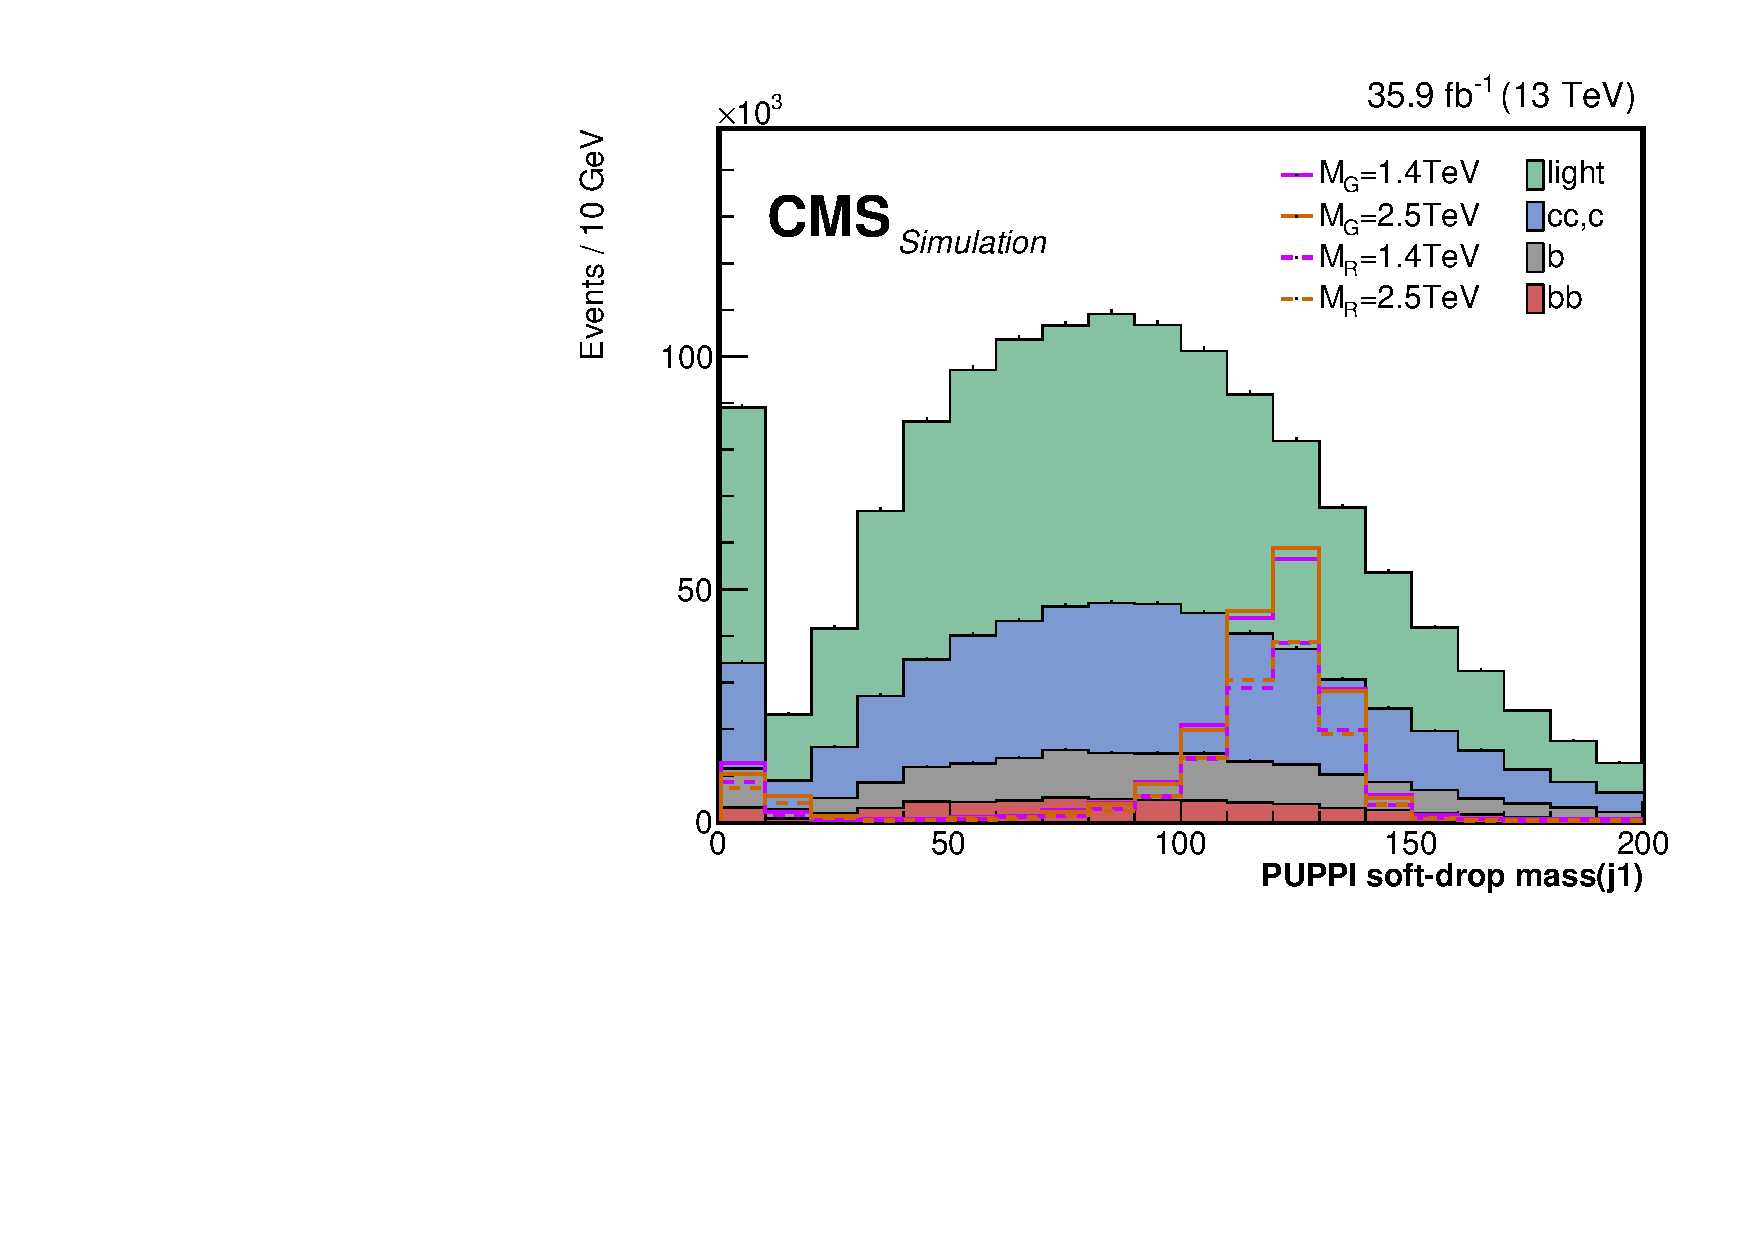
\includegraphics[width=0.5\textwidth]{Figures/MC_N1/puppiSDMassThea_j0.pdf} &
%    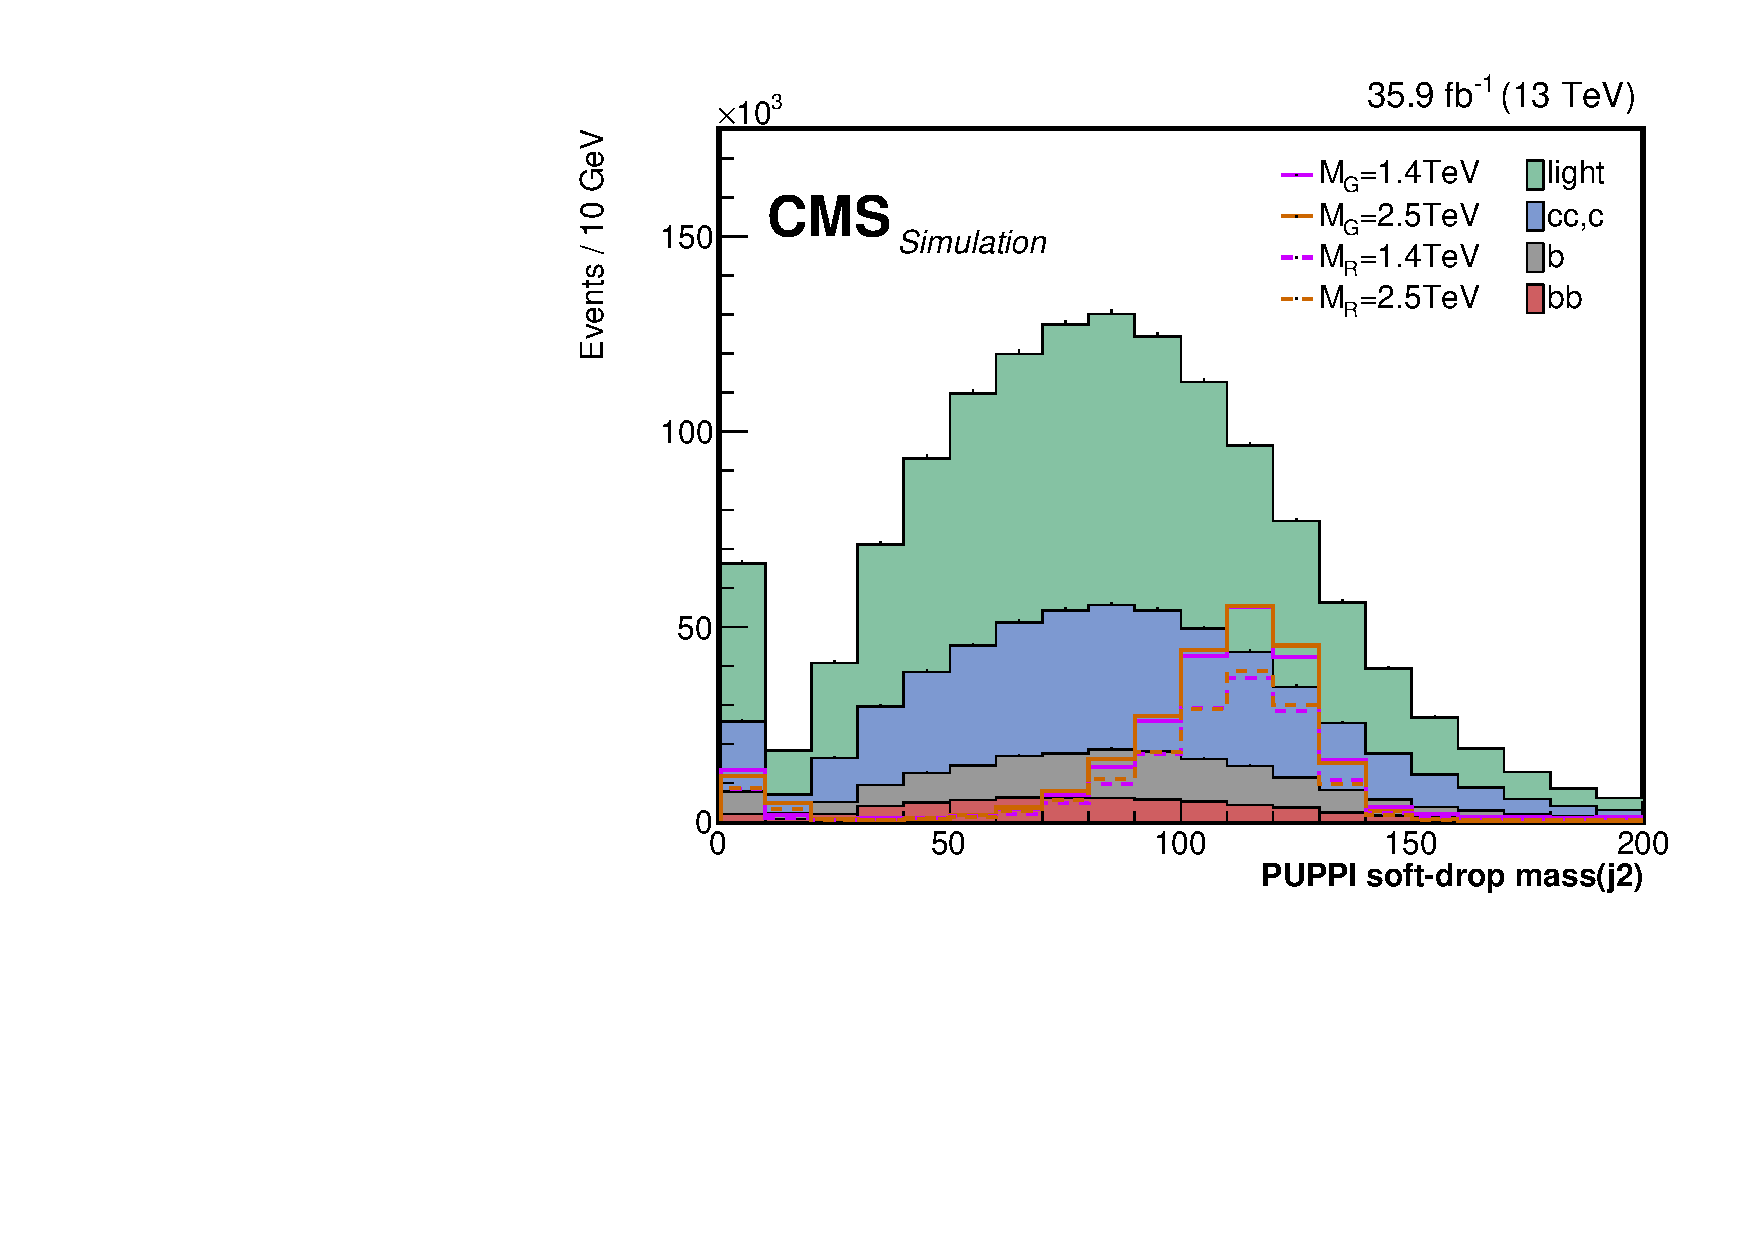
\includegraphics[width=0.5\textwidth]{Figures/MC_N1/puppiSDMassThea_j1.pdf} \\
%     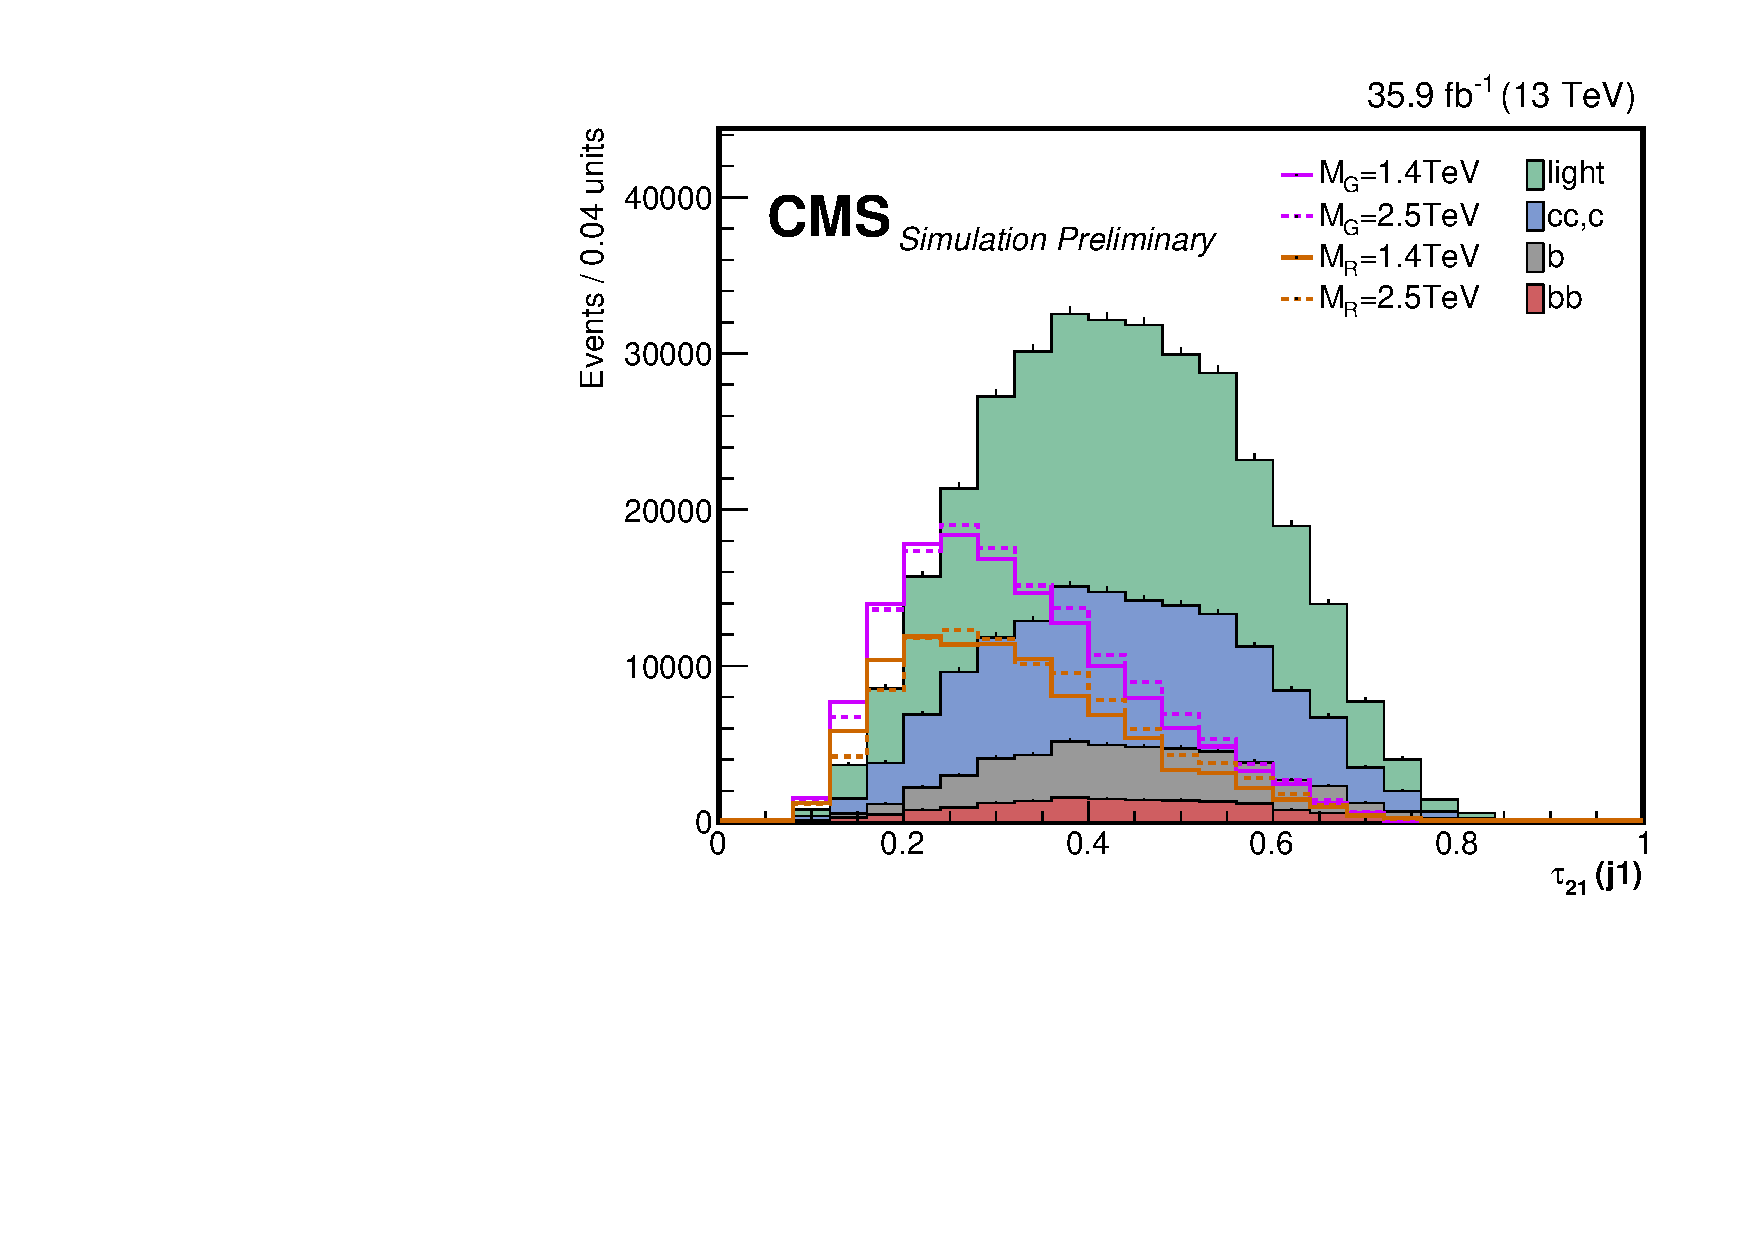
\includegraphics[width=0.5\textwidth]{Figures/MC_N1/puppiTau21_j0.pdf} &
%    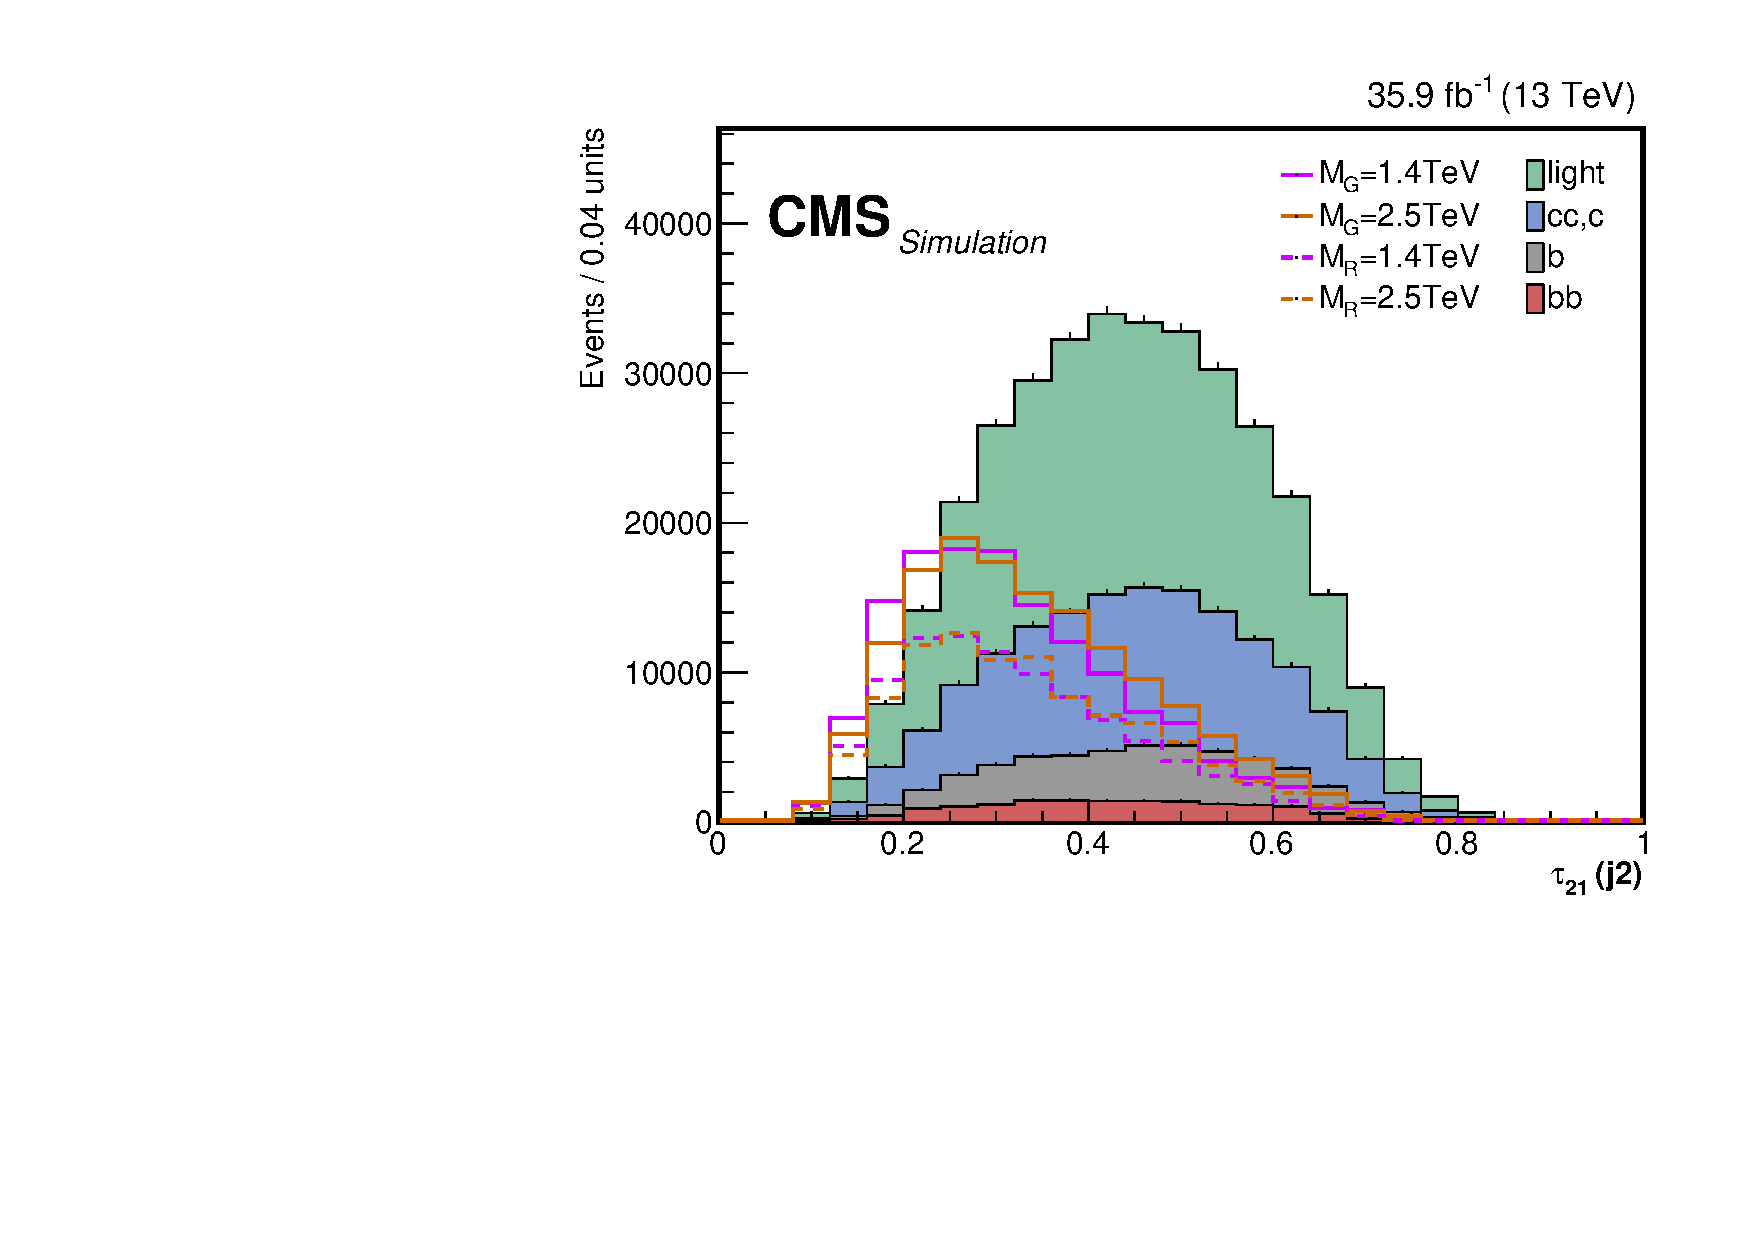
\includegraphics[width=0.5\textwidth]{Figures/MC_N1/puppiTau21_j1.pdf} \\
%     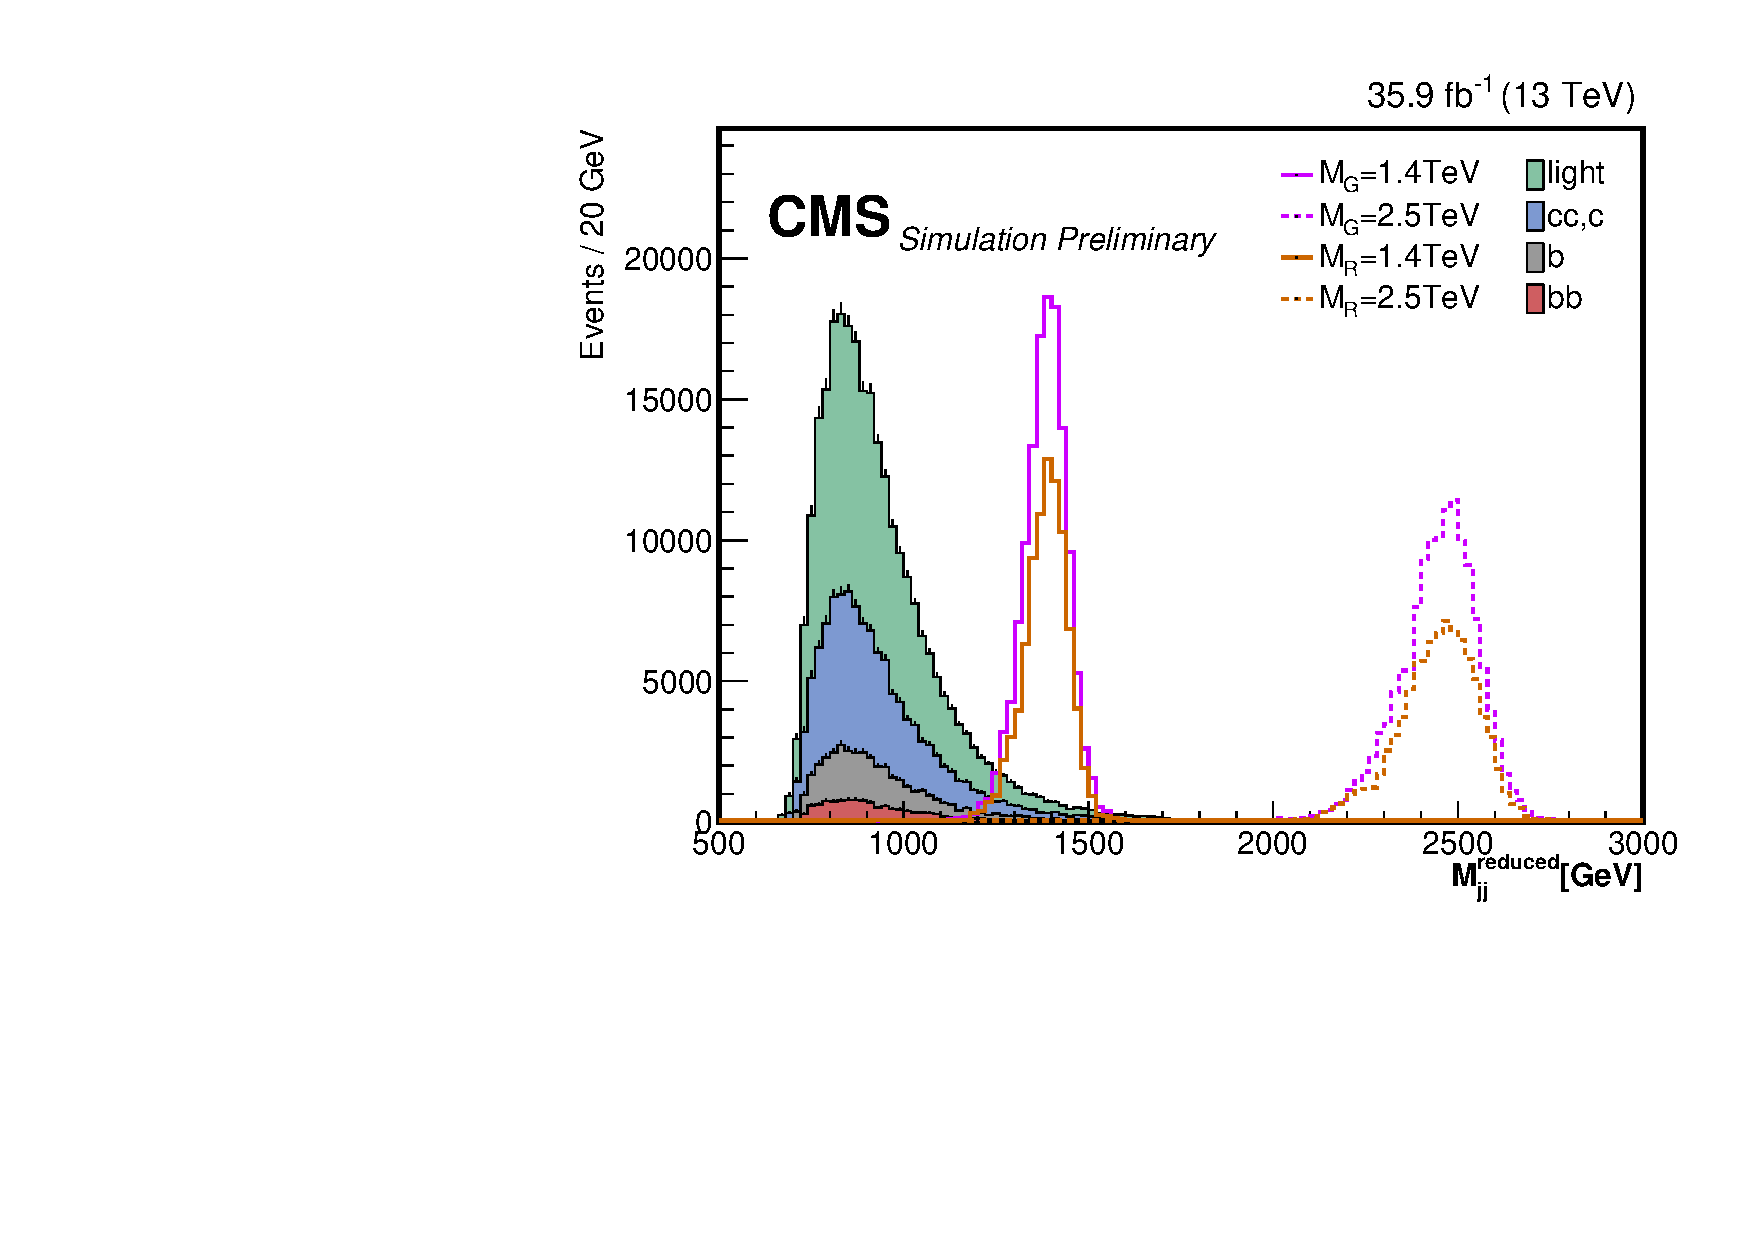
\includegraphics[width=0.5\textwidth]{Figures/MC_N1/totalMassRed.pdf} &
%    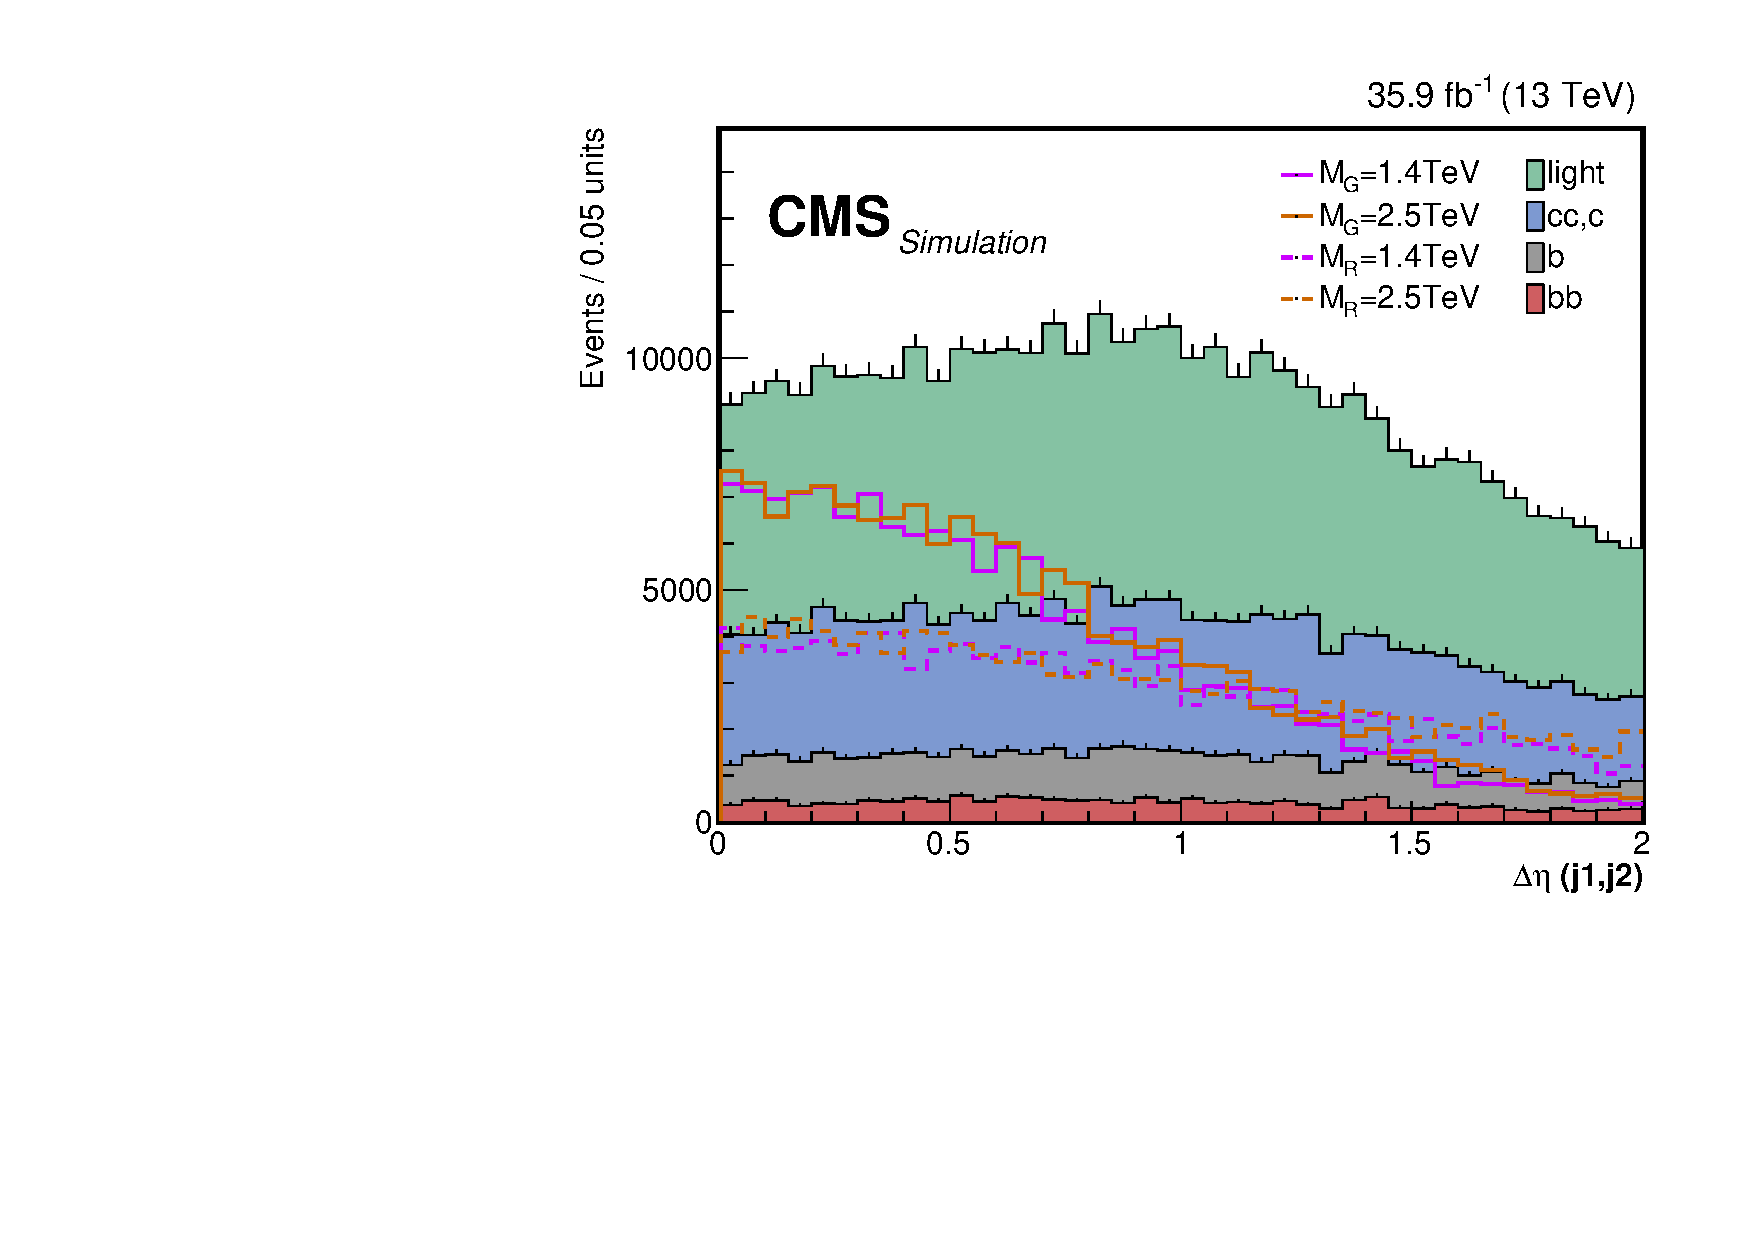
\includegraphics[width=0.5\textwidth]{Figures/MC_N1/deltaEta.pdf} \\
%  \end{tabular}
%  \caption{The comparison of signal and background. The signals of $M_{X}$ = 1.4 TeV and 2.5 TeV from both models are shown. The cross section is set to 20 pb in the figures. Multi-jet events are seperated into four categories summarized in the table 2.10. From top to buttom are the comparison of PUPPI soft-drop mass, $\tau _{21}$ of leading (left) and next leading (right) AK8 jet, the reduced mass (buttom left), and |$\Delta \eta $ (the two leading AK8 jets)| (buttom right).}
%  \label{fig:hvt_brs}
%\end{figure}